\documentclass[tikz]{standalone}
% Where `label=` puts its node (M4 step 4, D81): at an angle, at a direction
% word, and at an anchor of the node (north:, west:, north east:), on a
% rectangle, a diamond and a fit box on the background layer, as swimlane and
% group titles use them. Each label is named so its anchors can be compared.
\usetikzlibrary{positioning, fit, backgrounds, shapes.geometric}
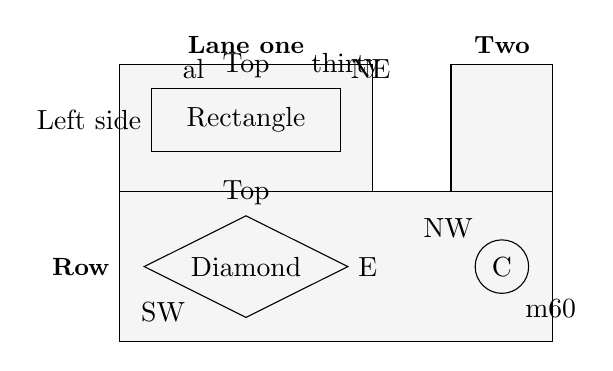
\begin{tikzpicture}[node distance=8mm and 16mm,
  lane/.style={draw, fill=gray!8, inner sep=3mm},
  lane title/.style={font=\bfseries\small}]
  \node[draw, minimum width=24mm, minimum height=8mm,
    label={[name=r1]north:Top}, label={[name=r2]west:Left side},
    label={[name=r3]north east:NE}, label={[name=r4]30:thirty},
    label={[name=r5]above left:al}] (r) {Rectangle};
  \node[draw, diamond, aspect=2, below=of r,
    label={[name=d1]north:Top}, label={[name=d2]south west:SW},
    label={[name=d3]east:E}] (d) {Diamond};
  \node[draw, circle, right=of d, label={[name=c1]north west:NW}, label={[name=c2]-60:m60}] (c) {C};
  \coordinate (lanes top) at (r.north);
  \coordinate (lanes bottom) at (d.south);
  \begin{scope}[on background layer]
    \node[lane, fit=(r) (d) (r |- lanes top) (r |- lanes bottom), label={[lane title, name=t1]north:Lane one}] (one) {};
    \node[lane, fit=(c) (c |- lanes top) (c |- lanes bottom), label={[lane title, name=t2]north:Two}] (two) {};
    \node[lane, fit=(d) (c), label={[lane title, name=t3]west:Row}] (row) {};
  \end{scope}
\end{tikzpicture}
